\PassOptionsToPackage{pdfpagelabels=false}{hyperref}
% \documentclass[useAMS,fleqn,usenatbib]{mnras} % fleqn left-aligns equations
\documentclass[useAMS,usenatbib]{mnras}
\pdfoutput=1 %for arxiv
\setlength{\topmargin}{-0.3in}

\usepackage{graphicx}
\usepackage{amsmath,amssymb,amstext}
\usepackage[T1]{fontenc}
\usepackage{ae,aecompl}
\usepackage[utf8]{inputenc}
% \usepackage{newtxtext,newtxmath}
\usepackage[figure,figure*]{hypcap}
\usepackage[dvipsnames]{xcolor}
\usepackage{bm}

\usepackage{xparse}

%% MINE
\usepackage{xspace} % smart spaces after custom \newcommand



%----------------------------------------
\newcommand{\qus}[1]{{\color{BrickRed}\textbf{[Q: }\textbf{#1}]}}
\newcommand{\arz}[1]{{\color{ForestGreen}\textbf{[Andrew: }\textbf{#1}]}}
\newcommand{\jan}[0]{{\color{TealBlue}\textbf{[Jeff: ]}}}
\newcommand{\tjr}[1]{{\color{Brown}\textbf{[Troy: }\textbf{#1}]}}


%-- Units
\newcommand{\Msun}{\mathrm{M}_{\odot}} % Msun
\newcommand{\Mstar}{\mathrm{M}_{\star}} % Mstar
\newcommand{\Msunh}{h^{-1}\mathrm{M}_{\odot}} % Msun/h
\newcommand{\hmpc}{\mathrm{h}^{-1}\mathrm{Mpc}} % Mpc/h
\newcommand{\kms}{\mathrm{km/s}}
\newcommand{\gev}{\mathrm{GeV}}

%-- Words
\newcommand{\lcdm}{$\Lambda$CDM\xspace}
\newcommand{\photoz}{photo-$z$\xspace}
\newcommand{\photozs}{photo-$z$'s\xspace}
\newcommand{\Photozs}{Photo-$z$'s\xspace}
\newcommand{\specz}{spec-$z$\xspace}
\newcommand{\speczs}{spec-$z$'s\xspace}
\newcommand{\z}{$z$\xspace}
\newcommand{\Z}{$Z$\xspace}


%-- Code packages
\newcommand{\mesa}{\texttt{MESA}\xspace}
\newcommand{\fortran}{\texttt{Fortran}\xspace}
\newcommand{\python}{\texttt{Python}\xspace}
\newcommand{\rockstar}{\texttt{ROCKSTAR}\xspace}
\newcommand{\halotools}{\texttt{Halotools}\xspace}
\newcommand{\corrfunc}{\texttt{Corrfunc}\xspace}
\newcommand{\glue}{Glue\xspace}
\newcommand{\xgboost}{\texttt{XGBoost}\xspace}
\newcommand{\gpz}{\texttt{GPz}\xspace}




%-- Figures and Equations
\newcommand{\equ}[1]{\[#1\]}
\newcommand{\nequ}[2]{\begin{equation}#1 \label{#2}\end{equation}}
\newcommand{\equin}[1]{\(#1\)}
\newcommand{\figscale}[4]{
% commands: width scale, path, caption, label
\begin{figure}[h]
    \centering
    \includegraphics[width=#1\textwidth]{#2}
    \caption{#3}
    \label{#4}
\end{figure}
}


\usepackage{url}

%% ENDMINE

%%%%%%%%%%%%%%%%%%% TITLE PAGE %%%%%%%%%%%%%%%%%%%

% Title of the paper, and the short title which is used in the headers.
% Keep the title short and informative.
\title[Asymmetric Dark Matter in Stars]{The Effects of Asymmetric Dark Matter on Stellar Evolution I: Spin-Dependent Scattering}

% The list of authors, and the short list which is used in the headers.
% If you need two or more lines of authors, add an extra line using \newauthor
\author[T.J. Raen et al.]{%
Troy J. Raen,$^{1}$\thanks{E-mail: troy.raen@pitt.edu},
Héctor Martínez-Rodríguez$^{1}$, 
Travis J. Hurst$^{2}$,
Andrew R. Zentner$^{1}$,\newauthor
Carles Badenes$^{1}$,
and Rachel Tao$^{3}$
\vspace*{12pt}
\\
% List of institutions
$^{1}$Department of Physics and Astronomy \& Pittsburgh Particle Physics, Astrophysics, and Cosmology Center (Pitt PACC),\\ University of Pittsburgh, Pittsburgh, PA 15260, USA\\
$^{2}$Department of Mathematics and Physics, Colorado State University -  Pueblo, Pueblo, C0, 81001 \\%Fixed my contact info. TJH
$^{3}$Department of Physics, Emory University, Atlanta, GA 30322
}
% These dates will be filled out by the publisher
\date{\today}

% Enter the current year, for the copyright statements etc.
\pubyear{2020}

% Don't change these lines
\begin{document}
\label{firstpage}
\pagerange{\pageref{firstpage}--\pageref{lastpage}}
\maketitle



% Abstract of the paper
\begin{abstract}
Most of the dark matter (DM) search over last few decades has focused on WIMPs but the viable parameter space is quickly shrinking. Asymmetric Dark Matter (ADM) is a WIMP-like DM candidate with slightly smaller masses and no present day annihilation, meaning that stars can capture and build up large quantities of it. The captured ADM can transport energy through a significant volume of the star. We investigate the effects of spin-dependent ADM energy transport on stellar structure and evolution in stars with \mrange in varying DM environments. We wrote a publicly available MESA module (footnote with repo link) that calculates the capture of DM and the subsequent energy transport within the star. We fix the DM mass to 5 GeV and the cross section to $10^{-37}$ cm${^2}$, and we study varying environments by scaling the DM capture rate. For stars with radiative cores ($\Mstar \lesssim 1.3 \Msun$), the presence of ADM flattens the temperature and burning profiles in the core, but the effect on MS lifetimes and observable properties is small. However, in higher mass stars, ADM energy transport shuts off the convection in the core, limiting the fuel available and therefore shortening MS lifetimes by as much as $~40\%$. This translates to changes in the luminosity and effective temperature of the MS turnoff in stellar population isochrones.
\end{abstract}

% Select between one and six entries from the list of approved keywords.
% Don't make up new ones.
\begin{keywords}
keyword1 -- keyword2 -- keyword3
\end{keywords}

%%%%%%%%%%%%%%%%%%%%%%%%%%%%%%%%%%%%%%%%%%%%%%%%%%







%%%%%%%%%%%%%%%%% BODY OF PAPER %%%%%%%%%%%%%%%%%%

\section{Introduction}
\label{sec:intro}

% \arz{I think I like $\mdm$ for the dark matter particle mass. The 
% problem with using $\chi$ is that it is heavily tied to the WIMP scenario because 
% in the case of a SUSY WIMP, $\chi$ is the symbol for the neutralino that might 
% be the dark matter. Thus, using $\chi$ suggests that SUSY WIMP scenario, which 
% we don't want to do.}

\arz{I added a number of references to "bib.bib." For some reason, I couldn't 
open "references.bib."}
\tjr{I will fix this.}

  A preponderance of the evidence suggests that approximately $84\%$ of the matter budget of the 
  universe consists of a form of non-baryonic dark matter that has yet to be identified. 
  \arz{Let's cite a few dark matter review articles here including Jungman+96, Bertone+2006, the 
  Cosmic Visions report. Let's also cite some of the standard references for constraints on 
  cosmological parameters, such as the Planck result.} In 
  the standard picture of cosmological structure formation, 
  galaxies form within the potential wells of 
  large, nearly virialized halos of dark matter \citep{white_rees78,blumenthal_etal84}. 
  If the dark matter interacts with standard model particles, 
  it can be captured by stars moving through dark matter halos 
  \citep{press_spergel85,krauss_etal85, gaisser_etal86, griest_seckel87}. 
  Once captured, continued scattering within the stellar interior contributes 
  to energy transport within the star, potentially altering its evolution \citep{Spergel1985EffectInterior, Zentner2011AsymmetricDwarfs} 
  \tjr{get a few more references} \arz{Good idea. Look for papers by Fabio Iocco, 
  Ian Shoemaker, Malcolm Fairbairn, Jordi Casanellas, Ilidio Lopez}\tjh{you can check my paper for references as well.}. 
  The significance of this energy transport depends on the following 
  properties (in addition to the properties of the star): 
  (1) the DM mass, $\mx$; 
  (2) the DM-nucleon scattering cross section, $\sigxn$; 
  and (3) the total number of DM particles captured by a star, $\Nx$, 
  which itself depends on $\sigxn$ as well as the local DM environment from 
which the particles are captured (see \S~\ref{sec:props}). 
We study the effects of energy transport by asymmetric dark matter 
(ADM, see below)
in stars of mass \mrange living within a variety of dark matter 
environments using the publicly available code 
Modules for Experiments in Stellar Astrophysics \citep[\mesa,][]{Paxton2011ModulesMESA}\tjh{I would cite the other MESA instrument papers here as well. I think there are 3 now.}.

  Evidence supporting the claim that $\sim$84\% of the matter in the universe is in 
  an unknown form of dark matter is abundant and varied, ranging from the 
  anisotropy of the microwave background radiation to formation and structures of galaxies. 
  \arz{cite reviews here.} 
  However, dark matter has never been observed in any way other than through its 
  gravitational influence and much remains to be discovered about its fundamental nature. 
  For several decades, the leading candidate has been the so called Weakly-interacting massive particle (WIMP). 
  The classic WIMP is a heavy ($\mx \sim 10^2-10^3 \gev$) thermal relic whose contemporary abundance is set 
  by its annihilation rate in the early universe \arz{cite e.g., Kolb and Turner textbook 
  or some other standard reference for the reader that needs a definition of a thermal relic}. 
  Therefore, WIMPs are thought to have a fairly well established ``standard'' annihilation 
  cross section \citep[e.g.,][]{steigman_etal12}\tjh{I would say "WIMPs have a weak-scale annihilation cross section". }. This annihilation, in turn, limits the number of particles 
  that can accumulate within a star 
  as the rate of capture of new dark matter particles 
  equilibrates with annihilation in the stellar interior \citep{krauss_etal85}. 
  Despite numerous ongoing terrestrial direct detection experiments \arz{cite LUX, CRESST, 
  and so on. maybe ask Brian Batell for references to the very latest results here.} and 
  efforts to detect dark matter indirectly through its annihilation products \arz{cite the FERMI, HESS, 
  and VERITAS results here as well as IceCube constraints on dark matter}, 
  dark matter has not been observed non-gravitationally. The 
  available parameter space for classic WIMPs is rapidly shrinking 
  \citep{Amole16} \tjr{Still need to refer to a constraint paper.}, 
  which has triggered a surge in research into alternatives to the long-favored WIMP.


  Asymmetric dark matter (ADM) is an alternative to the classic WIMP in which 
  the relic abundance of the dark matter particle is set by a primordial asymmetry 
  rather than via annihilation \citep[for a review, see][and references therein]{adm_review}. 
  If the baryon and dark matter asymmetries are 
  related, then such models have the appealing property that they explain 
  the fact that the contemporary dark matter and baryon abundances are 
  of the same order of magnitude, which is otherwise surprising because 
  these relic abundances are determined by unrelated physics in the WIMP 
  scenario. The variety of specific incarnations of ADM is broad, 
  but ADM models typically predict particle masses smaller than 
  the classic WIMP ($\mx \sim 1-10 \gev$) and no contemporary 
  dark matter annihilation due to the present-day absence of 
  dark matter anti-particles. 
  
  
  These predictions motivate studies to 
  constrain ADM indirectly through stellar astrophysics. The lack of 
  annihilation means that ADM may build up to very large
  quantities within stars because the capture of ADM is never countered 
  by annihilation. Meanwhile, the relatively low masses 
  compared to the classic WIMP mean captured ADM particles orbit within 
  a significant volume of the star, out to $\rx \sim X$ \arz{Put number here.} 
  for a Sun-like star, which means that they experience large differences 
  in ambient temperature 
  throughout their orbits and can thus transport energy outward from the 
  stellar core extremely efficiently \citep{Spergel1985EffectInterior}. 
  These features of ADM have already motivated research into the possibility that 
  ADM may alter stellar evolution 
  \citep[e.g.][]{Zentner2011AsymmetricDwarfs,iocco_etal12,vincent_etal15}.
  In this paper we undertake a study of the properties and evolution of 
  stellar populations within halos of ADM. In this first paper on the topic, 
  we further narrow our study to spin-dependent ADM-nucleus scattering. 
  Spin-independent ADM-nucleus scattering leads to behaviors that are 
  qualitatively distinct from spin-dependent scattering; therefore we will 
  present results for the former case in a forthcoming manuscript. 


  % \arz{How about this edit (starting with a new paragraph)?}
  %   The degree of stellar cooling induced by dark matter
  %   depends upon the following DM properties:
  %   1) the WIMP mass $m_x$;
  %   2) the WIMP-nucleon scattering cross section $\sigma_{xn}$;
  %   and 3) the total number of WIMPs captured by a star $N_x$.
  %   We will characterize stellar cooling using these parameters.
  %   As we will show below, our results are most relevant to a class
  %   of dark matter models known as {\em asymmetric dark matter} (ADM)
  %   \arz{Need some generic ADM citations here, start by looking in my paper.}
  %   The number of standard WIMP dark matter particles that can be captured
  %   within a star is limited by the fact that WIMP capture will come to
  %   equilibrium with WIMP mutual annihilation within the star. In ADM models,
  %   the dark matter does not annihilate because the dark matter consists entirely
  %   of dark matter particles and is completely devoid of dark matter antiparticles.
  %   For this reason, $N_x$ can grow very large in ADM models, enabling the
  %   effects of dark matter on stellar evolution to grow correspondingly large
  %   over the lifetime of a star. Consequently, our proposal is to use
  %   astrophysical studies of stellar populations to constrain ADM. In this first
  %   paper, we further narrow our study to spin-dependent ADM-nucleus scattering
  %   because spin-dependent and spin-independent scattering lead to qualitatively
  %   distinct behaviors. We will present results for spin-independent scattering
  %   in a forthcoming manuscript.
  %   \arz{My proposal is to cut the following if you like the above.}
  %   In so doing, we remain agnostic as to the fundamental theory of the
  %   dark matter and quantify
  %   Therefore we remain agnostic
  %   \tjr{this sounds good, but I think is not technically what I mean. Is this a common usage?}
  %   to most of the details of the WIMP model and focus on the relevant parameter space that
  %   is both allowed by experiment and effective at transporting energy in the star.

% \arz{I'm not sure I understand the purpose of the following paragraph. How does it advance our story? It seems 
% unnecessary to me.}
%   While we cannot directly observe stellar interiors, standard models have been developed and refined over the last century that match observations quite well. They are based on solving a set of coupled differential equations that describe energy and mass conservation, energy transport, and hydrostatic equilibrium using equations of state, tabulated opacities, and the (evolving) compositions of stellar interiors (see \citealt{Pols1990StellarEvolution} for details).
%   \arz{I would also cite some of the classic textbooks here, because most of what you are discussing is available in standard textbooks on stellar evolution. My favorite book is the bible of stellar evolution, Kippenhahn and Weigert, but there are several good books on this topic.}
%   % For future reference, we list several approximate scaling relations which are followed by MS stars in the standards models:
%   % \begin{align}
%   %   L \propto M^(3.5 to 4) \\
%   %   R \propto M \\
%   %   tau \propto M^-(2.5 to 3) \\
%   %   Tc \propto M^0.57 pp, M^0.21 cno (pols page 132)
%   % \end{align}

% \arz{I think we should move this more detailed discussion of low-mass vs. high-mass stars to the results 
% section. So, let's remove everything staring here ***}
%   Stars spend most of their lifetimes on the main sequence (MS), a near equilibrium state powered by hydrogen burning in the core. This conversion of hydrogen to helium happens via two main channels: the proton–proton (pp-) chain and the carbon–nitrogen–oxygen (CNO) cycle. The CNO cycle is much more sensitive to the temperature, as can be seen by the approximate scaling relations of the burning rates:
%   \begin{align}
%     \epspp &\propto T^4 \\
%     \epsCNO &\propto T^{18}
%   \end{align}
%   This has several important consequences:
%   \begin{enumerate}
%     \item The pp-chain (CNO cycle) dominates in stars with central temperatures, $\Tc$, less (greater) than $\approx 2 \times 10^7 \K$.

%     \item The stable stellar structures in the two regimes are different. In CNO-dominated stars, radiative transport is insufficient to carry such large amounts of energy away from the central burning region, requiring these stars to have convective cores. In contrast, pp-dominated stars are stable with purely radiative cores.

%     \item Smaller energy production rates in pp-dominated stars also means that DM energy transport can be significant at much lower values than in CNO-dominated stars.
%   \end{enumerate}

%   $\Tc$ generally increases with stellar mass, and the temperature threshold in (i) is equivalent to $\Mstar \approx 1.3 \Msun$. This means that our mass range includes two qualitatively distinct groups, which we will refer to as low-mass stars (\mrangelow) and high-mass stars (\mrangehigh) for the purposes of this paper \qus{Is this ok or should I really call them low-mass and intermediate-mass stars?}. \arz{*** and ending here. This can be moved.}



  We generally find that ADM captured by stars can cool stellar cores to a degree that can have potentially 
  observable effects on stellar populations. In general, the extra cooling due to ADM reduces the main sequence (MS) lifetimes 
  of stars and alters their subsequent evolution \qus{only through the horizontal branch, right? After that they evolve normally.}. We summarize our results on stellar lifetimes in Figure~\ref{fig:mstau} 
  and the net effect on stellar populations in the form of stellar isochrones in Figure~\ref{fig:isos_cb} in 
  \S~\ref{sec:results}. The effects of stellar cooling are particularly large in environments in which 
  the ambient dark matter density is high and velocity dispersion is low, such that the capture of 
  dark matter is extremely efficient. Thus, these effects will be largest in dwarf satellite galaxies 
  and high-redshift galaxies. 
  
  In the following section, we summarize the dependence of the capture rate of dark matter 
  within stars on both dark matter and stellar properties. In \S~\ref{sec:methods}, we describe
  our simulations of stellar evolution including cooling due to ADM. We present our results 
  in \S~\ref{sec:results}. We discuss our results and draw conclusions in \S~\ref{sec:conclusions}.
  
  
\arz{I commented out two paragraphs here. I don't think we need them.}  
%  We present our final results in the form of Hertzsprung–Russell (HR) diagrams\footnote{Note that an observer's HR diagram plots color versus magnitude while theorists use $\Teff$ and $L$ which captures the same information. \qus{do I need this footnote?}}. In Figure \ref{fig:tracks} we plot stellar tracks (properties are functions of time for a given stellar mass). In Figure \ref{fig:isos_cb} we plot isochrones (properties are functions of stellar mass for a given age).
%
%  The observed luminosity, $L$, and effective temperature, $\Teff$, of a MS star remain roughly constant over human time scales; however, these observables do vary as a function of mass, making star clusters feasible testing grounds for DM constraints. All stars in a cluster live in the same DM environment and are assumed to have formed from a single molecular cloud, meaning they have approximately the same age and metallicity. Given a stellar evolution model and an initial mass function for the cluster, its properties can be predicted and isochrones compared to observations. We leave quantitative constraints to future work since they will require in-depth analysis of stellar demographics \qus{and environments?}.
%
%
%


% \subsection{Observing Stellar Evolution}
%
%   \tjr{Are there other parts of the paper for which this is also true?}
%   \arz{The information in this section is all correct and you should hang on to it
%   for the purposes of writing your thesis document, but... I would say that this
%   information is not necessary in a journal article. So, I would get rid of the
%   subsection heading and reduce this section to one, short paragraph.
%   I think that we can say that
%   we cast our final results into the form of H-R or color-magnitude diagrams and that
%   we defer taking this all the way to a constraint for a future paper. The reason for
%   deferring is simply that extracting an actual constraint from observational data
%   requires a great deal of work on stellar demographics that suffices to constitute a
%   publication of its own.}
%
%   Ultimately, the effects we calculate can be compared to observations to further constrain DM properties. We leave this comparison to future work, but will briefly describe the process in order to focus our results.
%
%   Stellar evolution is best observed using Hertzsprung–Russell (HR) diagrams\footnote{Note that an observer's HR diagram plots color versus magnitude while theorists use T$_{\rm{eff}}$ and L which captures the same information.} of star clusters. All stars in the cluster are assumed to have formed from a single molecular cloud and therefore to have approximately the same metallicity and age. For this reason these diagrams are also called isochrones. Given a stellar evolution model and an initial mass function for the cluster, their properties can be predicted and compared to observations.
%
%   Since the MS is a near equilibrium state, with gravitational contraction balanced by outward radiation pressure from nuclear burning, the observed luminosity, L, and effective temperature, T$_{\rm{eff}}$, remain roughly constant at values which increase with the star's total mass. Then MS stars lie roughly along a line with negative slope in an HR diagram (see Figure \ref{fig:stellarHR}).
%
%   As the core hydrogen supply depletes, the local burning rate must also decrease and the star leaves the MS. With less radiation pressure to counter gravity, the core contracts and the temperature rises. Once the temperature just outside the depleted core is sufficiently high, the hydrogen in that region ignites and the star enters a period of hydrogen shell burning. (This process happens quickly in  high mass stars and gradually in low mass stars, see Section \ref{sec:results} for details.) The shell burning region acts as a mirror and evolve up and to the right as they leave the MS \tjr{needs better explanation}. High mass stars have much higher central burning rates and so they burn through their hydrogen supply much more quickly. MS lifetimes are then inversely proportional to mass, and so a cluster's age can be determined by the location of this MS turn-off on the isochrone.
%
%   % %--------------------
%   % % stellar HR plots
%   % \begin{figure*}
%   % \centering
%   %   \includegraphics[width=\textwidth]
%   % %   {plots/HR_1_and_3p5_Msun.png}
%   % {plots/HR.png}
%   %   \caption{\label{fig:stellarHR}HR diagrams of the evolution of $1\Msun$ and $3.5\Msun$ stars. Only \nodm and c6 are shown for brevity. Marked positions correspond to the time the central hydrogen mass fraction falls below a threshold: ZAMS: 0.71, IAMS: 0.3, H-3: $10^-3$. (ZAMS and IAMS are used in Dotter.) Both models settle onto the MS at the same position in the HR plane, but move through the MS in different ways. NOTE: The data is cut: removed most of pre-MS and after MS turnoff. These cuts make it easier to see what I'm trying to show, but I'm not sure that my specific choices were the best. We should discuss.
%   %   }
%   % \end{figure*}
%   % %--------------------


%--------------
\section{Dark Matter Properties and Capture in Stars}
\label{sec:props}

  Probing the parameter space of ADM with simulations of stellar evolution is computationally expensive. 
  Consequently, we show results for a representative set of ADM parameters chosen to: 
  (1) make the effects of ADM on stellar evolution significant; 
  and (2) remain consistent with contemporary constraints on dark matter properties. 
  For our models we choose $\mx = 5 \gev\ (\approx 5\mprot)$ and a spin-dependent 
  scattering cross section of $\sigxp = 10^{-37} \cmsq$, where the subscript, p, refers to protons.
  Hereafter we will discuss ADM-proton scattering since protons are the only nuclei in MS stars with both a significant abundance and a net spin.
  We assume that ADM self-interactions 
  are negligible throughout; however, it is likely that self-interactions would lead to enhanced 
  cooling \citep[e.g.,][]{Zentner2009High-energySun} and exploring such models would 
  constitute a potentially interesting follow-up to this work.


  \tjr{Need something here on current m$_x$ and $\sigma_x$ constraints.}
  \arz{Yes, we need something here. It should just be a sentence saying that 
  these parameters are just below the contemporary constraints on spin-dependent 
  dark matter-nucleon scattering and give a citation to the latest result. 
  I'm guessing you got this from Brian already, but the Cosmic Visions report
  from last year gives a nice summary along with links to all of the relevant
  experiments.}

  The energy transported by dark matter is proportional to the amount of ADM within the star. 
  In ADM models, in which annihilation of dark matter is negligible, the number 
  of dark matter particles within the star at any given time, $t$, is given by $\Nx = \Cx t$ 
  where $\Cx$ is the capture rate. We use the capture rate from \citet{Zentner2011AsymmetricDwarfs}, 
  which is a simplified form valid for dark matter particle masses 
  $\mx \lesssim 20 \gev$ \citep[see][ for more complete capture rates]{Gould1992CosmologicalAnnihilations,Zentner2009High-energySun}:
%
  \begin{align}
  \begin{split}
    \label{eq:capturerate}
    \Cx =\ & \Csun
    \Big(\frac{\rhox}{0.4 \gev \cmcinv}\Big)
    \Big(\frac{270 \kms}{\bar{v}}\Big) \\
    & \times \Big(\frac{\sigxp}{10^{-43} \cmsq}\Big) \Big(\frac{5 \gev}{\mx}\Big) \\
    & \times \Big(\frac{v_{\mathrm{esc}}}{618 \kms}\Big)^2
    \Big(\frac{\Mstar}{\Msun}\Big)
  \end{split}
  \end{align}
%
  where $\Csun = 5 \times 10^{21} \sinv$, 
  $\rhox$ is the DM density in the stellar environment,
  $\bar{v}$ is the velocity dispersion of dark matter particles 
  in the stellar neighborhood, and $v_{\mathrm{esc}}$ is the escape speed from the 
  surface of the star.
  % This capture rate depends on both the properties of the ADM and the dark matter halo in which the star lives.

  The first line of Eq.~(\ref{eq:capturerate}) gives the dependence of the capture rate on the stellar environment. 
  Both $\rhox$ and $\bar{v}$ are properties of the local stellar environment and are degenerate with one another in Eq.~(\ref{eq:capturerate}); a higher ambient density 
  of dark matter leads to a higher rate of dark matter capture, while a lower relative velocity between 
  the star and the infalling dark matter leads to a higher probability for capture. 
  Therefore it is convenient to parameterize a star's local dark matter 
  environment by an overall factor \citep{Zentner2011AsymmetricDwarfs,Hurst2015},
%
  \begin{equation}
  \gb = \bigg(\frac{\rhox}{0.4 \gev \cmcinv}\bigg) \Bigg(\frac{270 \kms}{\bar{v}}\Bigg).
  \label{eq:gammab}
  \end{equation}
%
 \tjh{I made the parenthesis around  bigger with slash bigg and slash Bigg. This encloses all the text and looks a little better imo.} Normalized in this way, 
  $\gb$ specifies the capture rate, $\Cx$, relative to 
  the rate that would be realized in the solar neighborhood for the same star. 
  From this point on we will characterize a star's dark matter environment using 
  $\gb$ due to the fact that density and velocity dispersion are degenerate in 
  Eq.~(\ref{eq:capturerate}). 
  In general, we will be most interested in values of $\gb > 1$, so we will refer 
  to $\gb$ as the environmental boost factor. 
  % It is most natural to think of $\Gamma_B$ as quantifying the dark matter environment. For example,
  A value of $\gbzero$ describes a stellar environment with no dark matter
  (hereafter referred to as `standard models' and labeled `\nodm'), 
  and $\gbone$ describes the solar neighborhood. 
  A value of $\gbpow{2}$ may specify an environment in 
  which the dark matter density is 100 times that in the 
  solar neighborhood at the same velocity dispersion, 
  an environment in which the velocity dispersion is 1/100 
  that of the solar neighborhood at the same density, 
  or any of an infinite number of other possible combinations.
 


It is interesting to consider the range of $\gb$ values that would be considered reasonable. If the distribution of 
dark matter within galaxies such as the Milky Way follows a profile that diverges as the 
\citet[][NFW]{nfwprofile} density profile, then one might expect to find a dark matter environment near the Galactic center with
densities significantly higher than the local value and velocity dispersions significantly
lower than the local value, giving $\gb \gg 1$.
However, stellar populations near the Galactic Center
are difficult to observe and any assumption about the dark matter density profile in the 
inner regions of any galaxy must be considered highly speculative. 
Interestingly, Local Group dwarf galaxies are extremely dark matter-dominated 
and have well constrained dark matter profiles and velocity dispersions. 
In some cases, the Local Group dwarfs have densities $\sim 2-3$ orders 
of magnitude higher than the dark matter density in the Solar neighborhood 
and have velocity dispersions that are at least $\sim 2$ orders of magnitude 
smaller than the local value. This suggests that values of $\gb \sim 10^{5-6}$ 
could be realized within Local Group dwarfs and has the further merit that 
$\gb$ within Local Group dwarfs can be \qus{measured?} more precisely in the future. 
\arz{TO DO: Address $\gb$ in high-redshift galaxies.}
Finally, while we have focused on the boost paramter $\gb$ as a proxy for 
the dark matter environment in which a star is embedded, we note that values 
of $\gb \ne 1$ can also be mimicked through dark matter physics. 
In particular, 
dark matter self-interactions can enhance the capture rates of dark 
matter within stars \citep{Zentner2009High-energySun}.


%----------------------------------------------
\section{Methods}
\label{sec:methods}

  We study the impact of dark matter on the evolution of 
  \mrange stars through the thermal pulse (or equivalent) phase using the publicly-available code Modules for Experiments in Stellar Astrophysics \citep[\mesa,][]{Paxton2011ModulesMESA}. \mesa models stellar evolution by simultaneously solving coupled differential equations that describe stellar structure and composition. We base our models on the \mesa inlist used in \citet{Choi2016mesaModels}\footnote{\url{http://waps.cfa.harvard.edu/MIST/}} (see also \citealt{Dotter2016MesaIsochrones}); however, we turn off rotation and diffusion and use a hard net \todo{explain this better}.

  The size of each time step in a \mesa model can vary by orders of magnitude, and so output for different \mesa runs may contain information at drastically different times. To generate isochrones we must interpolate output from a range of initial stellar masses, with all other parameters held constant. We accomplish this using code written by \citet{Dotter2016MesaIsochrones}\footnote{\url{https://github.com/aarondotter/iso}}. It takes a set of \mesa runs and uses key evolutionary phases to guide the interpolation. This helps to ensure that phases with shorter time scales are properly represented in the interpolation.

%---------
\subsection{Energy Transport by Dark Matter}
\label{sub:energytransport}

  The energy transported by captured ADM can, in principle, be computed by solving the Boltzmann equation; however, this strategy is too computationally intensive to combine with a full-scale simulation of the evolution of stellar structure. To reduce the computational costs of our simulations, we estimate ADM energy transport using the approximations of \citet{Spergel1985EffectInterior}. In particular, we assume a Maxwellian phase-space distribution for the ADM and calculate an orbit-averaged temperature, $\Tx$, by requiring that the distribution satisfy the first moment of the Boltzmann equation. This amounts to a requirement on energy conservation: ADM should neither inject nor remove a net energy from the star. The rate of energy transfer (per unit mass) from dark matter to protons is then
  % \tjr{use \ is full space, '\,' '\.' . can also use begin{eqnarray} }
  %
  \begin{align}
  \begin{split}
  \epsx(r) =\ & 8\ \sqrt[]{\frac{2}{\pi}} \frac{\nx(r) \nprot(r)}{\rho(r)} \frac{\mx \mprot}{(\mx+\mprot)^2} \sigxp\\
  & \times \Big(\frac{\mprot k \Tx + \mx k T(r)}{\mx \mprot}\Big)^{1/2} k (\Tx - T(r)),
  \label{eq:xheat}
  \end{split}
  \end{align}
  %
  where $n(r)$ is a number density, $\rho(r)$ is the mass density, $k$ is Boltzmann's constant, and the subscript p refers to protons. \citep[See][for a detailed derivation]{Spergel1985EffectInterior}.

  Generally, $\nprot$, $\nx$, and $T$ all peak at the center (exceptions noted below), so the energy transport is most efficient here. The number density 
  of dark matter particles, $\nx$ increases in proportion with $\Nx$, so we can expect the effects to increase with both $\gb$ and stellar age through the MS, while hydrogen is abundant. As a star leaves the MS, $\nprot$ drops in the core and spin-dependent ADM energy transport is greatly diminished because there are relatively few protons left with which dark matter may scatter\footnote{This is one of the primary reasons that spin-dependent and spin-independent scattering gives qualitatively distinct results. As the star burns H on the MS, the number of protons is reduced, reducing the importance of spin-dependent scattering processes. In the case of spin-independent scattering, the effect gets more important as helium 
  is produced from H burning during the MS.}. A standard MS temperature profile decreases monotonically with distance from the star's center, but it can become temporarily inverted when ADM moves large amounts of energy away from the center (requires $\gb \gg 1$) \qus{should I mention any standard conditions that cause this? degeneracy?}. \arz{You can give guidelines 
  if you know them. But if not, it is ok.}

  The sign of $\epsx(r)$ is given by the final term in (\ref{eq:xheat}), $\Tx - T(r)$, which is used to define an ADM characteristic radius, $\rx$, implicitly as
  %
  \begin{align}
    T(r=\rx) = \Tx.
  \end{align}
  %
  Then dark matter takes energy from $r < \rx$ and deposits it at $r > \rx$ for a standard MS temperature profile. With our chosen ADM parameters we see typical values:
  %
  \begin{align}
    \rx & \sim \mathcal{O}(0.1 \Rstar) \\
    \lx = (\sigxp \nprot)^{-1} & \sim\mathcal{O}(1 \Rstar)
  \end{align}
  \todo{check that the data agree with these estimates}
  %
  where $\lx$ is the ADM mean free path (implying that it completes several orbits between scattering events). These values allow dark matter to travel much larger distances than photons or ions within the star (which have $l \lesssim 10^{-10} \Rstar$) and to traverse qualitatively distinct 
  regions of the star. This large mean free path is what enables dark matter 
  to serve as such an effective coolant despite being far less numerous than either photons or ions \citep{Press1985EffectInterior}. \qus{should I mention anything else here? like seeing a significant temperature gradient or something related to the convection effects?} \arz{I think this is good.}

  % \arz{The preceding statement is probably not true, right? Near $r=0$, the temperature gradient is very small, so energy transport probably is not maximally efficient at the center of the star.} \tjr{What I mean is that the magnitude of the extra heat is largest at r=0, see Fig \ref{fig:m1p0_a}, top right plot. This is generally, but not always, true. Is it the word "efficient" that's a problem?}
  \todo{orphaned: dm probes temp diffs over large portion of star. so temp gradient shallow at center dm energy transport can still be efficient. contrary to standard stellar evolution.}

  \todo{check that old plots are xluminosity and not xheat.}
  
  
  \arz{We should probably mention that our (your) software module 
  will be made available through the standard MESA portal. Do you 
  also want to point to a github page for your module?}
  \tjr{Yes. Is the abstract the right place to do both of those things?}


%------------------------------------------
\section{Results}
\label{sec:results}

In standard stellar evolution, with no influence from dark matter, stars with \mrange naturally split into two groups with qualitatively different structures, based on the dominant channel through which they burn hydrogen. The dominant channel is determined by the core temperature, with the transition happening at $\Tc \sim 2 \times 10^7 \K$, which corresponds to $\Mstar \sim1.3 \Msun$.

Low mass stars burn hydrogen primarily through the proton-proton (pp) chain for which the burning rate scales with temperature very roughly as $\epspp \propto T^4$. In these stars, the transport of energy away from the core burning region is dominated by photon diffusion. Energy transport in the cores of such stars is said to be radiative.

High mass stars are dominated by the carbon-nitrogen-oxygen (CNO) cycle for which the burning rate scales much more strongly with temperature as $\epsCNO \propto T^{16-20}$. In CNO-dominated stars, radiative energy transport is insufficient to carry away the energy produced by hydrogen burning. Consequently, these high-mass stars have convective cores.

\arz{Cite one or more standard references on stellar structure here. I am partially to Kippenhahn, but whatever you like is fine.}.

In \S~\ref{sub:lowmass} and \S~\ref{sub:highmass}, we will consider results for high-mass stars and low-mass stars separately and we will demonstrate that ADM has distinct effects on the evolution of the two groups.


%------------------------------------------
\subsection{Low-Mass Stars}
\label{sub:lowmass}

  % 1.0Msun, energy and temperature
  \begin{figure}
    \centering
    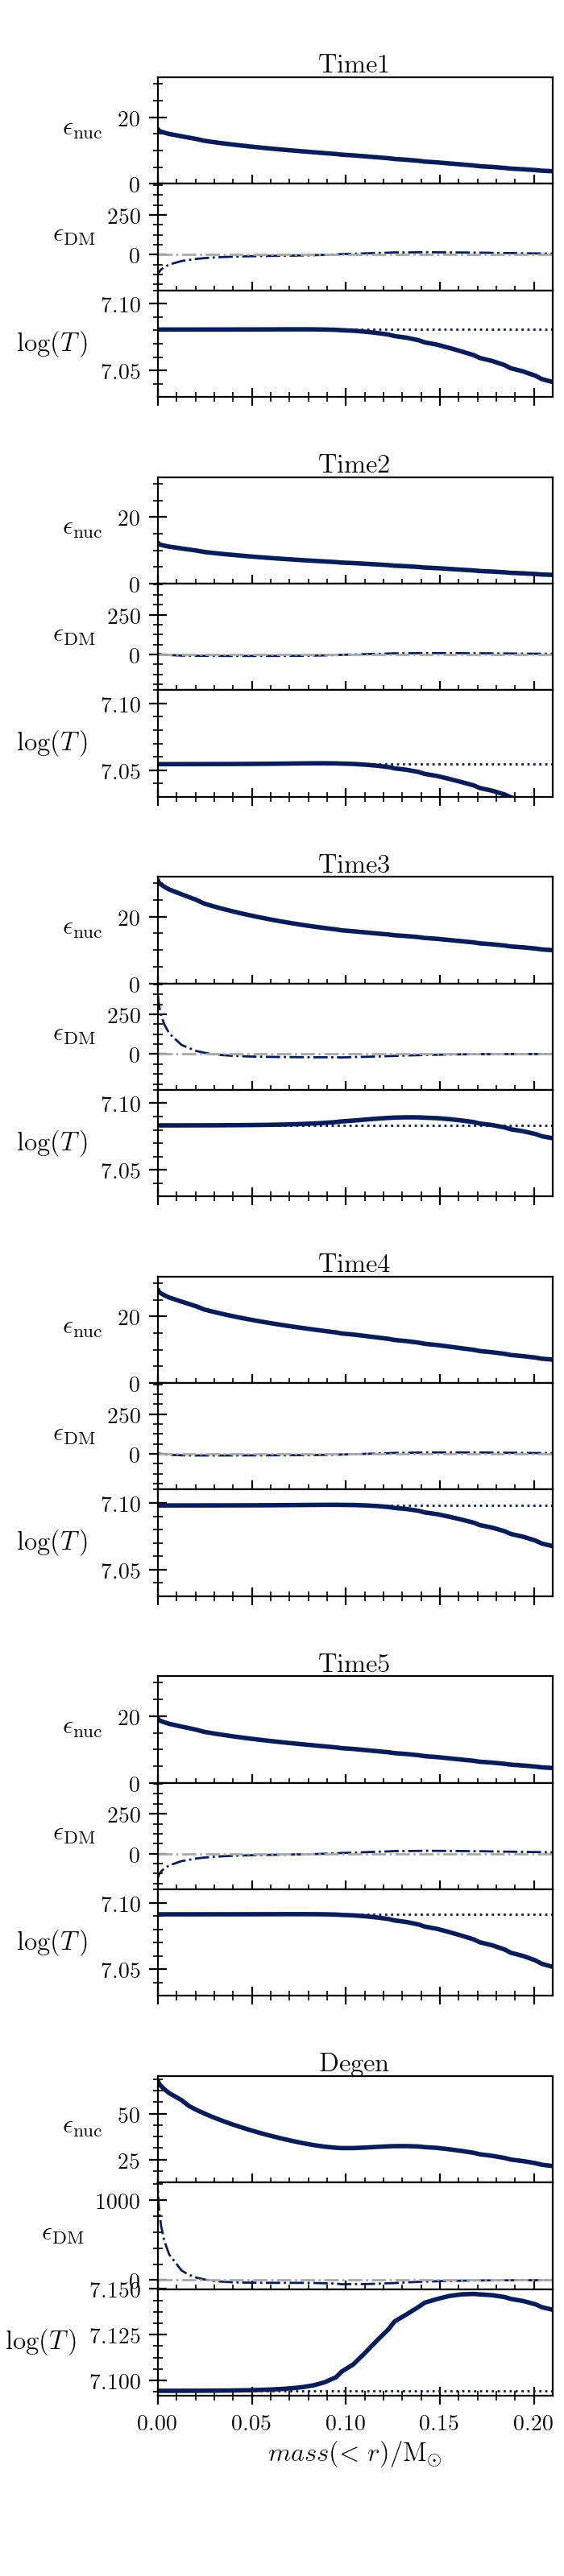
\includegraphics[width=0.47\textwidth]{plots/m1p0c6.png}
    \caption{PLACEHOLDER. $1.0 \Msun$ profiles for \nodm (grey) and $\gbpow{6}$ (dark blue) models. In each set of 3 panels, the top 2 are the same as in Figure~\ref{fig:m3p5}. The third panel is the temperature in [K], with the characteristic ADM temperature, $\Tx$, shown as a thin dotted line. ADM energy transport decreases hydrogen burning in the core and pushes the burning into a shell more quickly than the reference models. The reduced central burning causes the $\gbpow{3}$ model to live slightly longer than the \nodm model.
    }
    \label{fig:m1p0c6}
  \end{figure}


Standard model stars in the mass range \mrangelow have relatively low central temperatures and so are powered primarily by the pp chain, which is much less sensitive to the temperature than burning via the CNO cycle. This means the burning does not peak as strongly at the center and radiative transport is sufficient to carry the energy flux, so the core is radiative. Without the mixing provided by convection, hydrogen depletes first at the very center and the burning shifts gradually outward into a shell.

As seen in Fig.~\ref{fig:m1p0c6}, energy transport by large amounts of ADM cause flatter temperature profiles than those seen in the \nodm model. This reduces the burning rate in the center (where ADM is removing energy) and increases it in a shell (where ADM deposits energy).


%------------------------------------------
\subsection{High-Mass Stars}
\label{sub:highmass}

  % 3.5Msun profiles, energy and convection
  \begin{figure}
    \centering
    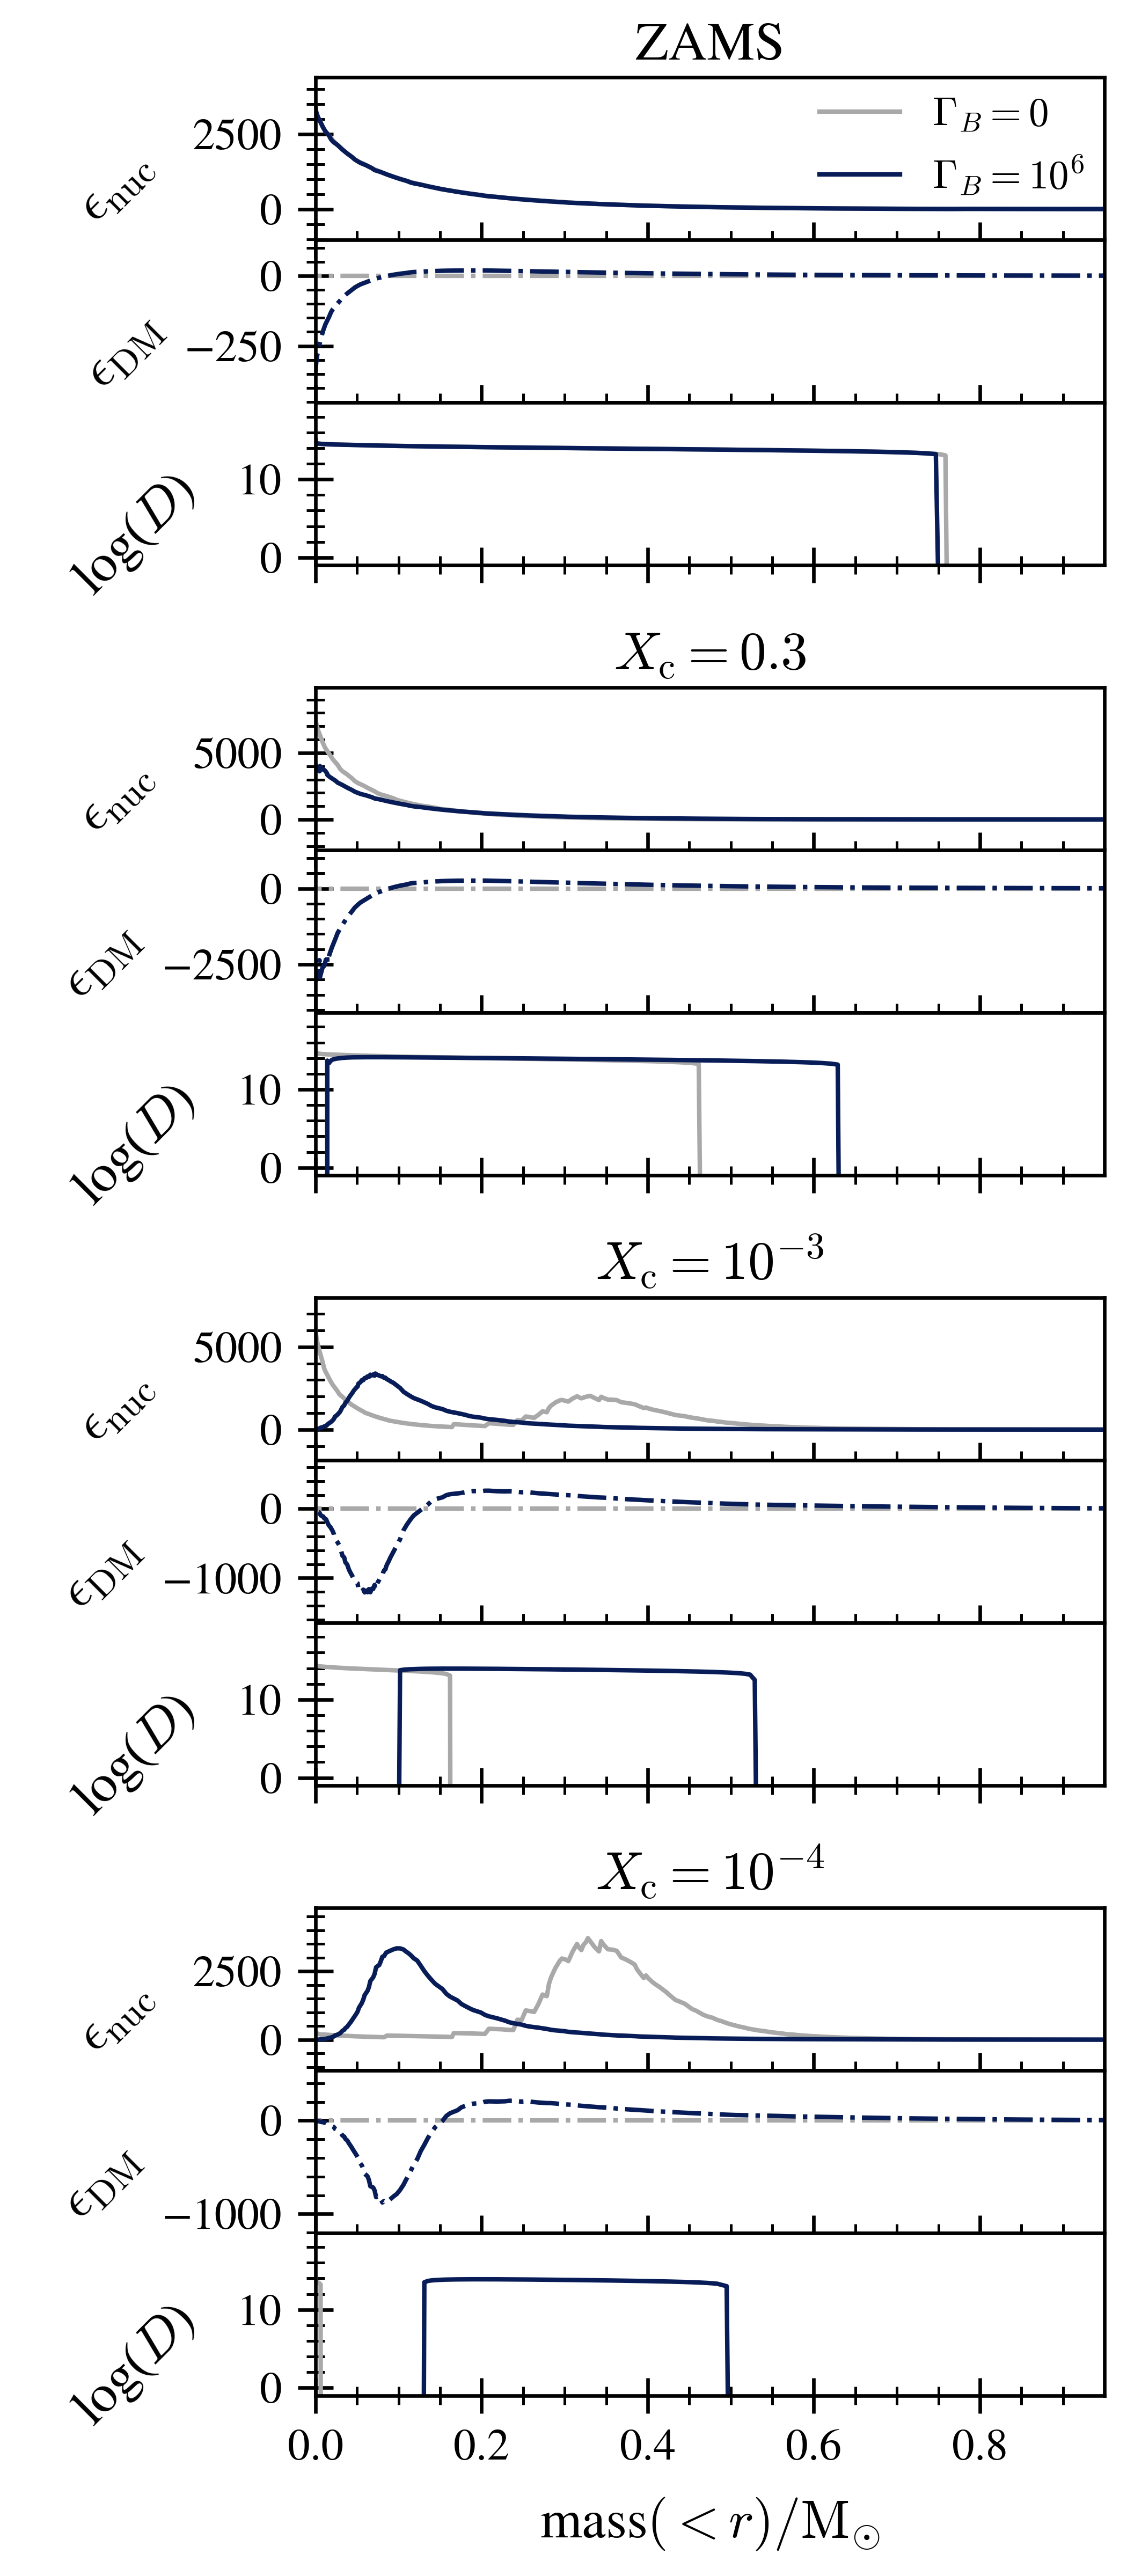
\includegraphics[width=0.47\textwidth]{plots/m3p5.png}
    \caption{$3.5 \Msun$ profiles for \nodm (grey) and $\gbpow{6}$ (dark blue) models. Each set of 3 panels shows stellar profiles of the stars at different evolutionary phases indicated by the fraction of hydrogen in the center, $X_c$, which decreases as the star evolves. The profiles in each panel are: 1) $\epsnuc$, the nuclear burning rate in [erg/g/s], 2) $\epsx$, the rate at which DM transports energy (negative values indicate that energy is being removed), also in [erg/g/s], 3) D, the diffusion coefficient for convective + overshoot mixing in [cm$^2$/s]. In the \nodm model the convective core retreats \textit{toward} the center over time, and the burning rate peaks at the center until the end of the main sequence when the burning rate drops dramatically and a shell of strong burning suddenly appears. In the $\gbpow{6}$ model, convection at the very center shuts off early in the MS and a convective shell retreats \textit{away} from the center over time. The peak burning rate shifts gradually outward, following the inner edge of the convective shell.
    }
    \label{fig:m3p5}
  \end{figure}

In standard models, MS stars with $\Mstar \gtrsim 1.3 \Msun$ are powered primarily by the CNO cycle.
This has several important consequences:
(1) the burning rate is much higher than in pp-dominated stars;
(2) the burning rate is extremely sensitive to core temperature;
and (3) stellar cores must be convective in order to carry away the energy produced by core hydrogen burning.
Once hydrogen throughout the convective zone is depleted, the burning rate rapidly decreases, and the star loses more energy at its surface than is being generated by burning. Gravity temporarily dominates over the pressure support from burning and the star contracts until the internal temperature increase is sufficient to ignite hydrogen in a shell outside the depleted core. See Figure~\ref{fig:m3p5}.

If a star captures enough ADM, the combination of dark matter + radiative energy transport becomes sufficient to carry the flux from nuclear burning. Convection disappears from the center first (where ADM energy transport is most efficient) and retreats away from the core, into a narrowing shell. Without convective mixing, the central hydrogen supply depletes (I don't think this is the right reason) and the burning also shifts into a shell, following the lower boundary of the convective zone. This can be seen in the time progression (down the page) of the $\gbpow{6}$ (dark blue) model in Figure~\ref{fig:m3p5}. The shift to shell burning is more similar to the behavior of standard low mass models.


%------------------------------------------
\subsection{Main Sequence Lifetimes}
\label{sub:mstau}

% mstau plot
\begin{figure*}
  \centering
  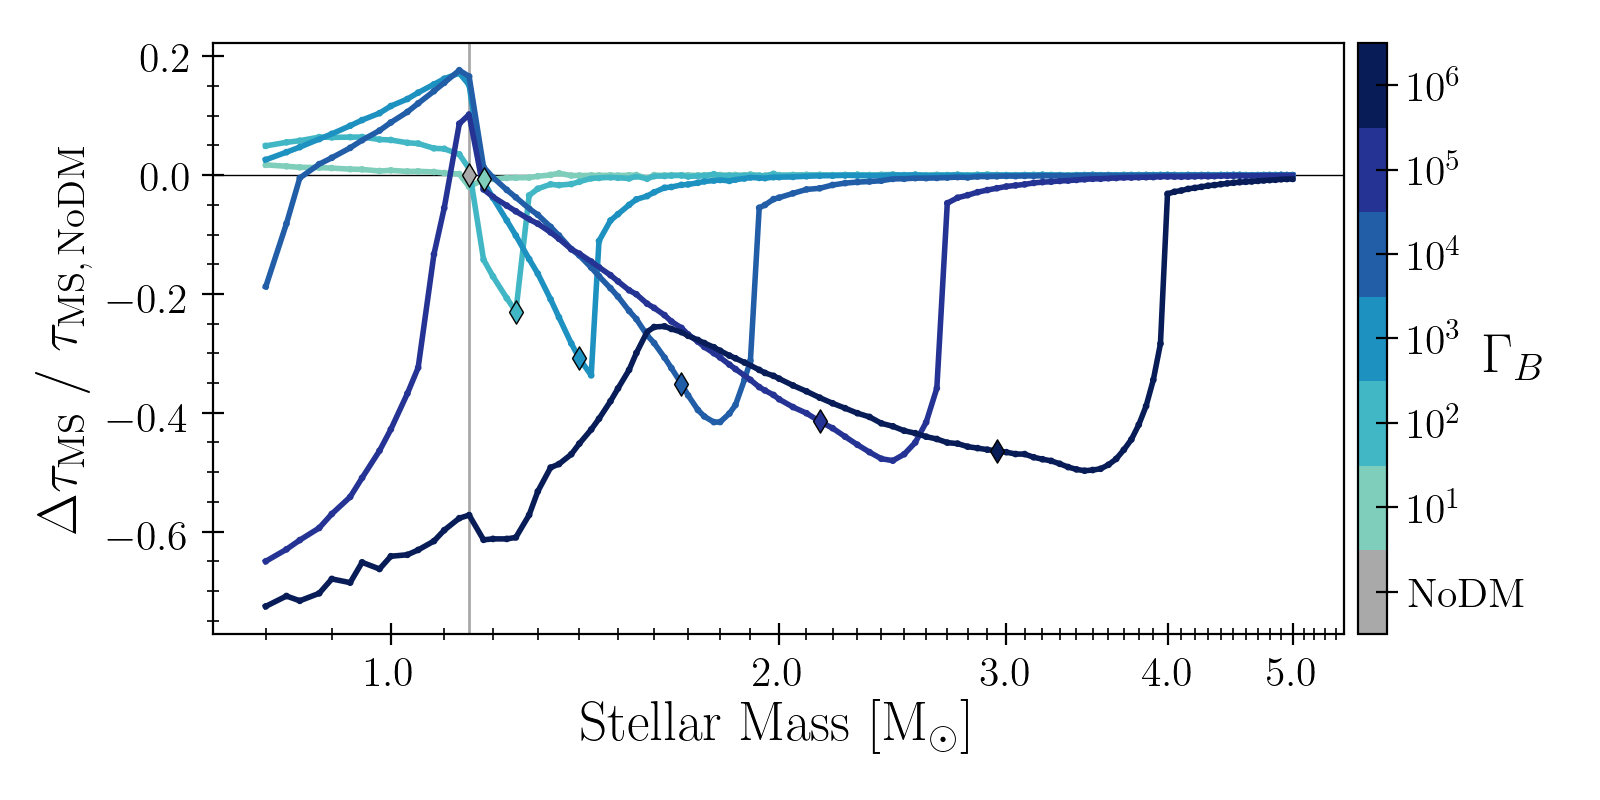
\includegraphics[width=\textwidth]{plots/mstau.png}
  \caption{The presence of ADM tends to shorten MS lifetimes relative to models with no dark matter.
  Diamonds mark the transition from radiative to convective cores (left to right). For the purposes of this figure this is defined as the lowest \Mstar for which the average (over the MS) mass of the convective core is greater than 0.01 Mstar. This transition is also marked by a vertical line for the \nodm model since this is what splits the low and high mass groups. Stars to the right of this line have decreased lifetimes due to a reduction in the size of the convective core, which reduces the amount of hydrogen available for burning. The effect abruptly disappears as stellar lifetimes become shorter than the time required to build up a sufficient amount of ADM. Stars to the left of the vertical line show mixed behavior. Those with lower $\gb$ have increased lifetimes due to decreased burning rates. Those with high $\gb$ show little change.
  }
  \label{fig:mstau}
\end{figure*}

In Fig.~\ref{fig:mstau} we show the effects of ADM on main sequence (MS) lifetimes relative to a standard \nodm star of the same mass. We have defined the MS to end when the fractional abundance of hydrogen in the center, $X_c$, falls below $10^{-3}$ (check the number, MIST defines TAMS = 10^-12). $X_c$ declines rapidly at the end of the MS, so our results are not strongly affected by the exact choice.

Lifetimes of low mass stars, which have radiative (not convective) cores even in \nodm models, are not greatly affected by ADM. Models with intermediate \gammaB values have their lifetimes extended by up to $~20\%$ because the DM energy transport reduces the temperature in the center, which in turn reduces the burning rate. Models that capture large amounts of ADM (high \gammaB values) have very little change in their MS lifetimes. (why? Perhaps the burning rate in the shell is high enough, and the settling happens fast enough that helium ash accumulates in the core at the same rate as in no DM models?)

ADM tends to shorten the lifetimes of high mass stars ($\Mstar \gtrsim 1.3 \Msun$), an effect that increases with \gammaB. In \nodm models, the central convection zone extends beyond the burning region, giving the star a source of fresh nuclear fuel as hydrogen from outside of the core is mixed into the center. Since ADM shuts off convection in the center, the star no longer gets this influx of unburnt hydrogen, therefore it has less fuel to burn and so it leaves the MS faster than the \nodm models. Note that the appearance of the convective core shifts to higher masses with increasing \gammaB (diamonds in Fig.~\ref{fig:mstau}) due to larger amounts of ADM which can carry larger energy fluxes. The effects disappear abruptly as $\Mstar$ approaches $5 \Msun$ because stellar lifetimes (which scale as $\Mstar^{-2.5}$ (check exact number)) quickly become too short for a sufficient amount of ADM to build up in the star (recall that the ADM capture rate scales linearly with $\Mstar$).


%------------------------------------------
\subsection{Isochrones}
\label{sub:isochrones}

% isochrones plots
\begin{figure*}
  \centering
  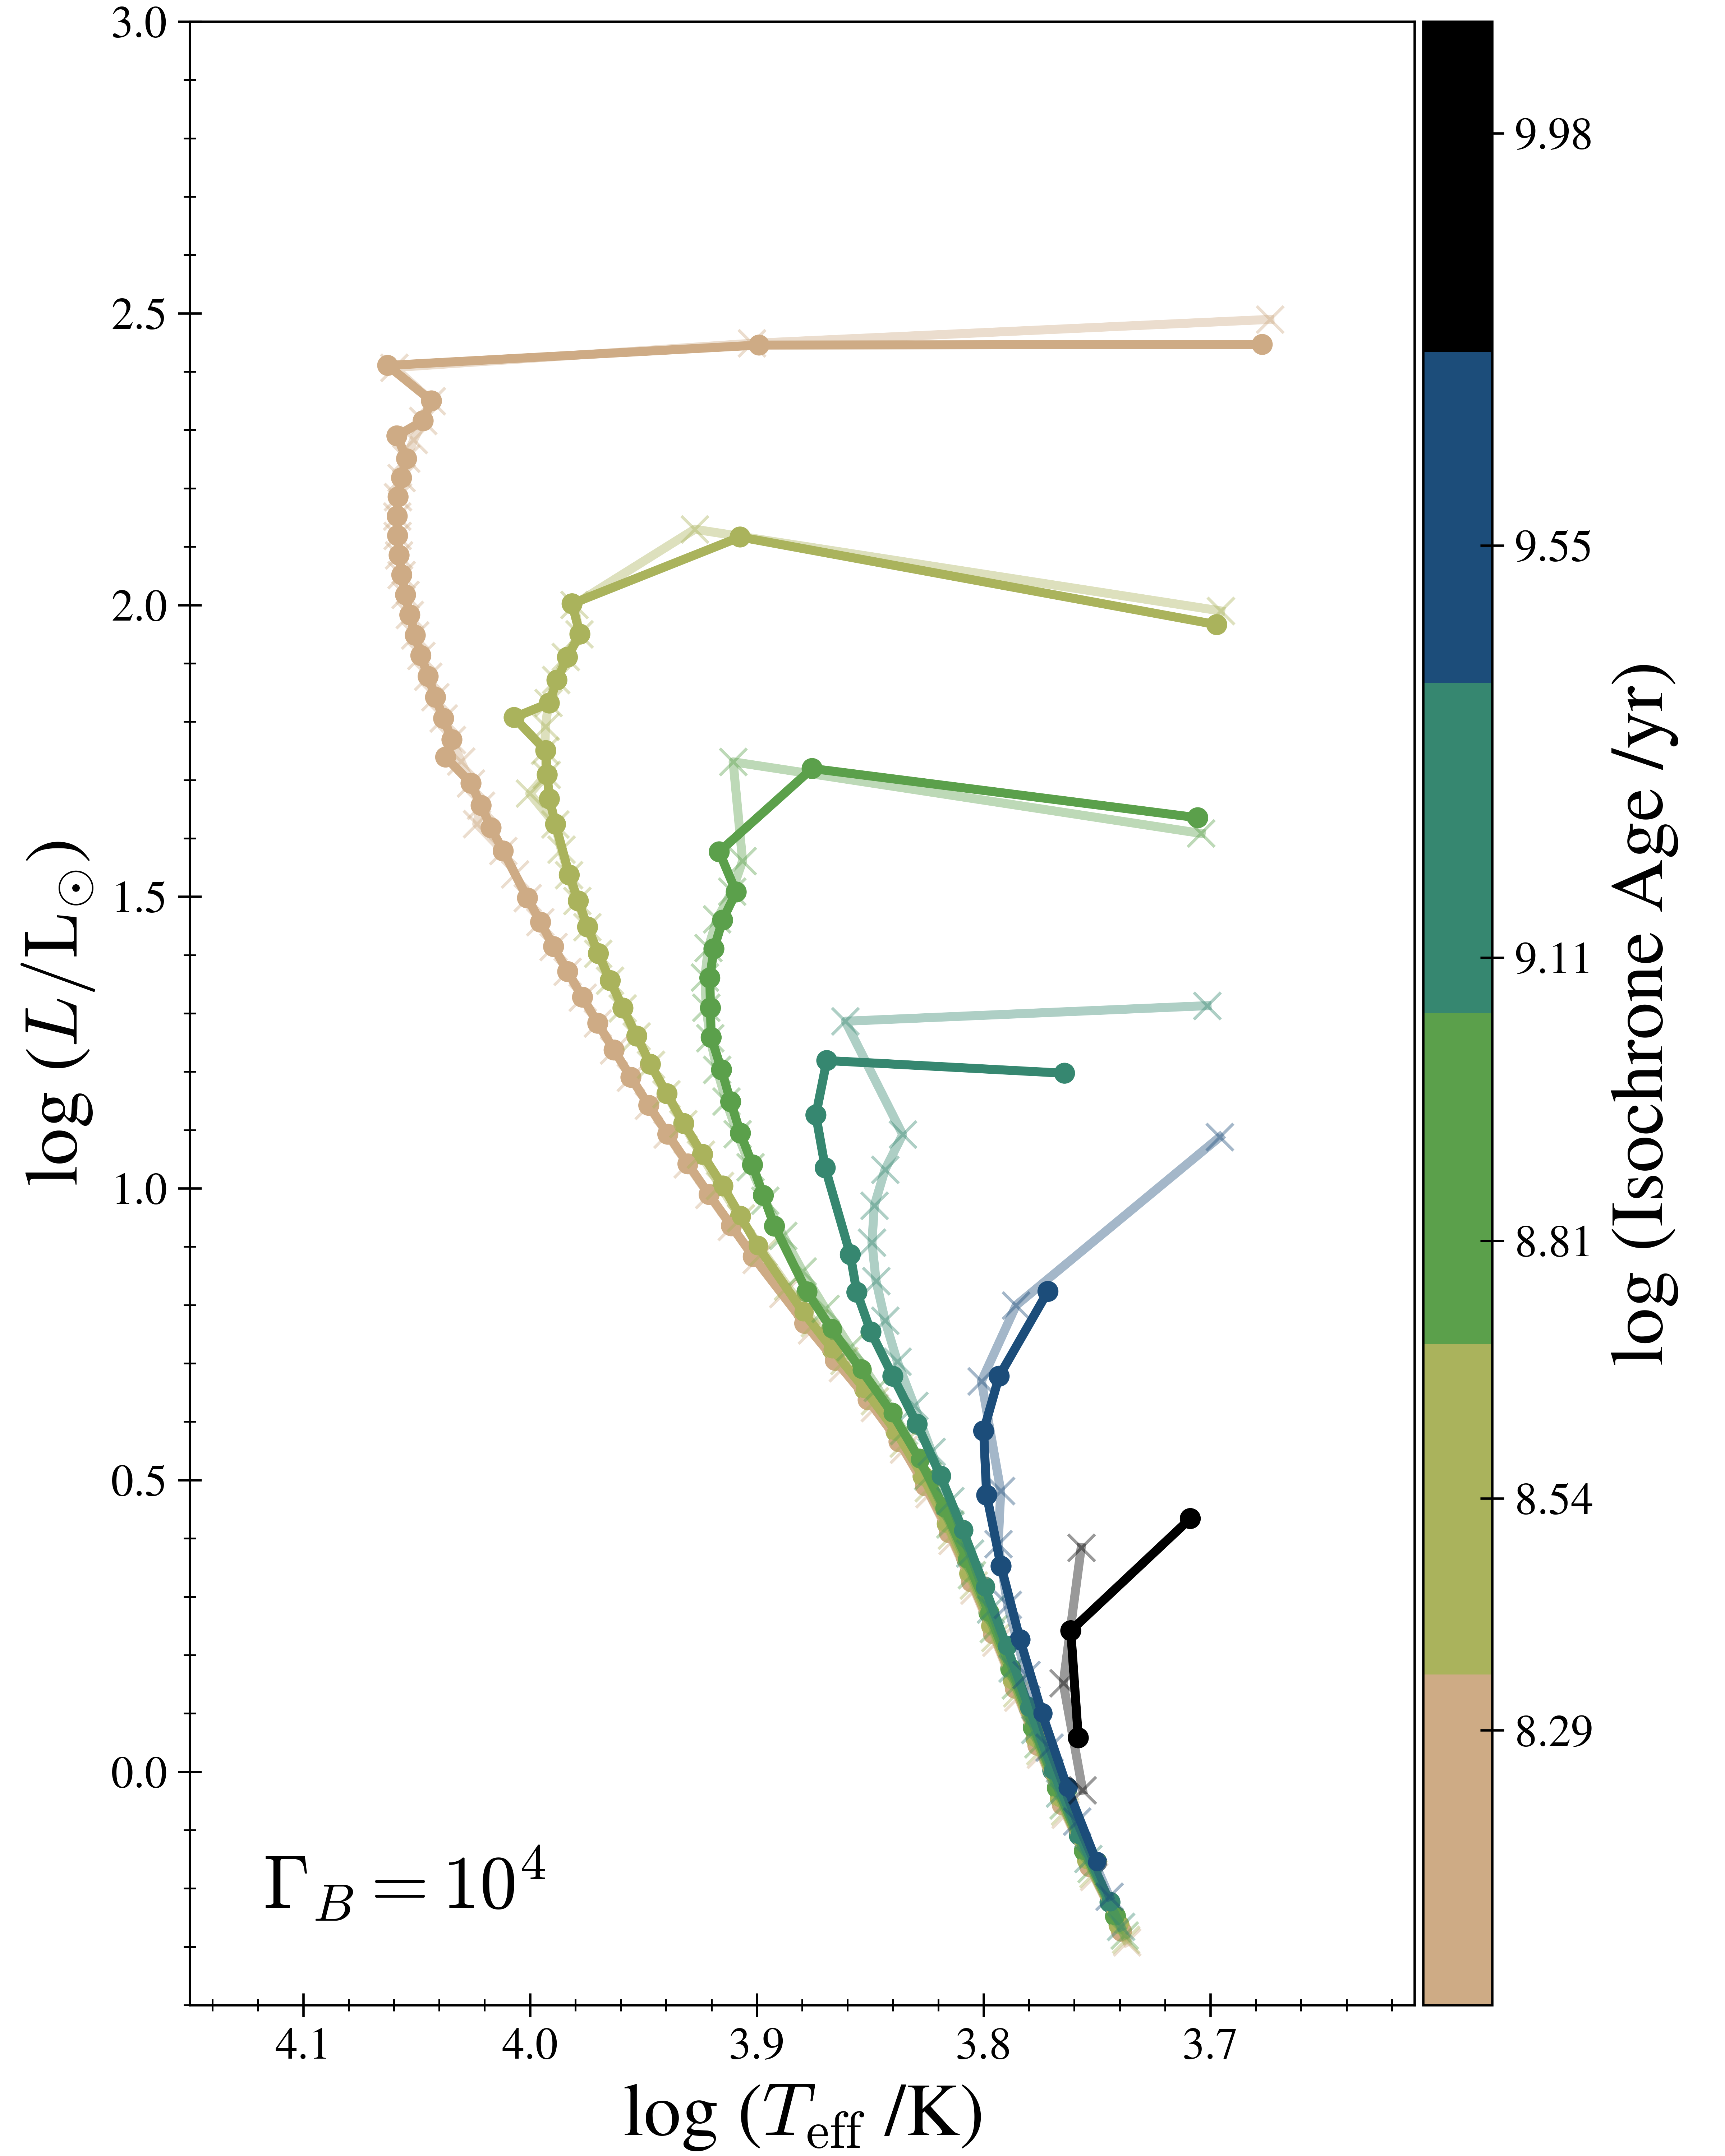
\includegraphics[width=\textwidth]{plots/isos_cb4.png}
  \caption{$\gbpow{4}$ isochrones with \nodm models overplotted as thin lines. Triangles mark $3.5 \Msun$, circles mark $1.0 \Msun$. The positions of the markers here are very similar to the \nodm case (not shown). Gaps in the data are due to the difficulty interpolating in regions where the evolution of lower mass stars is \textit{faster} than that of stars with slightly higher masses (see \S~\ref{sub:isochrones}).
  }
  \label{fig:isos_cb4}
\end{figure*}

\begin{figure*}
  \centering
  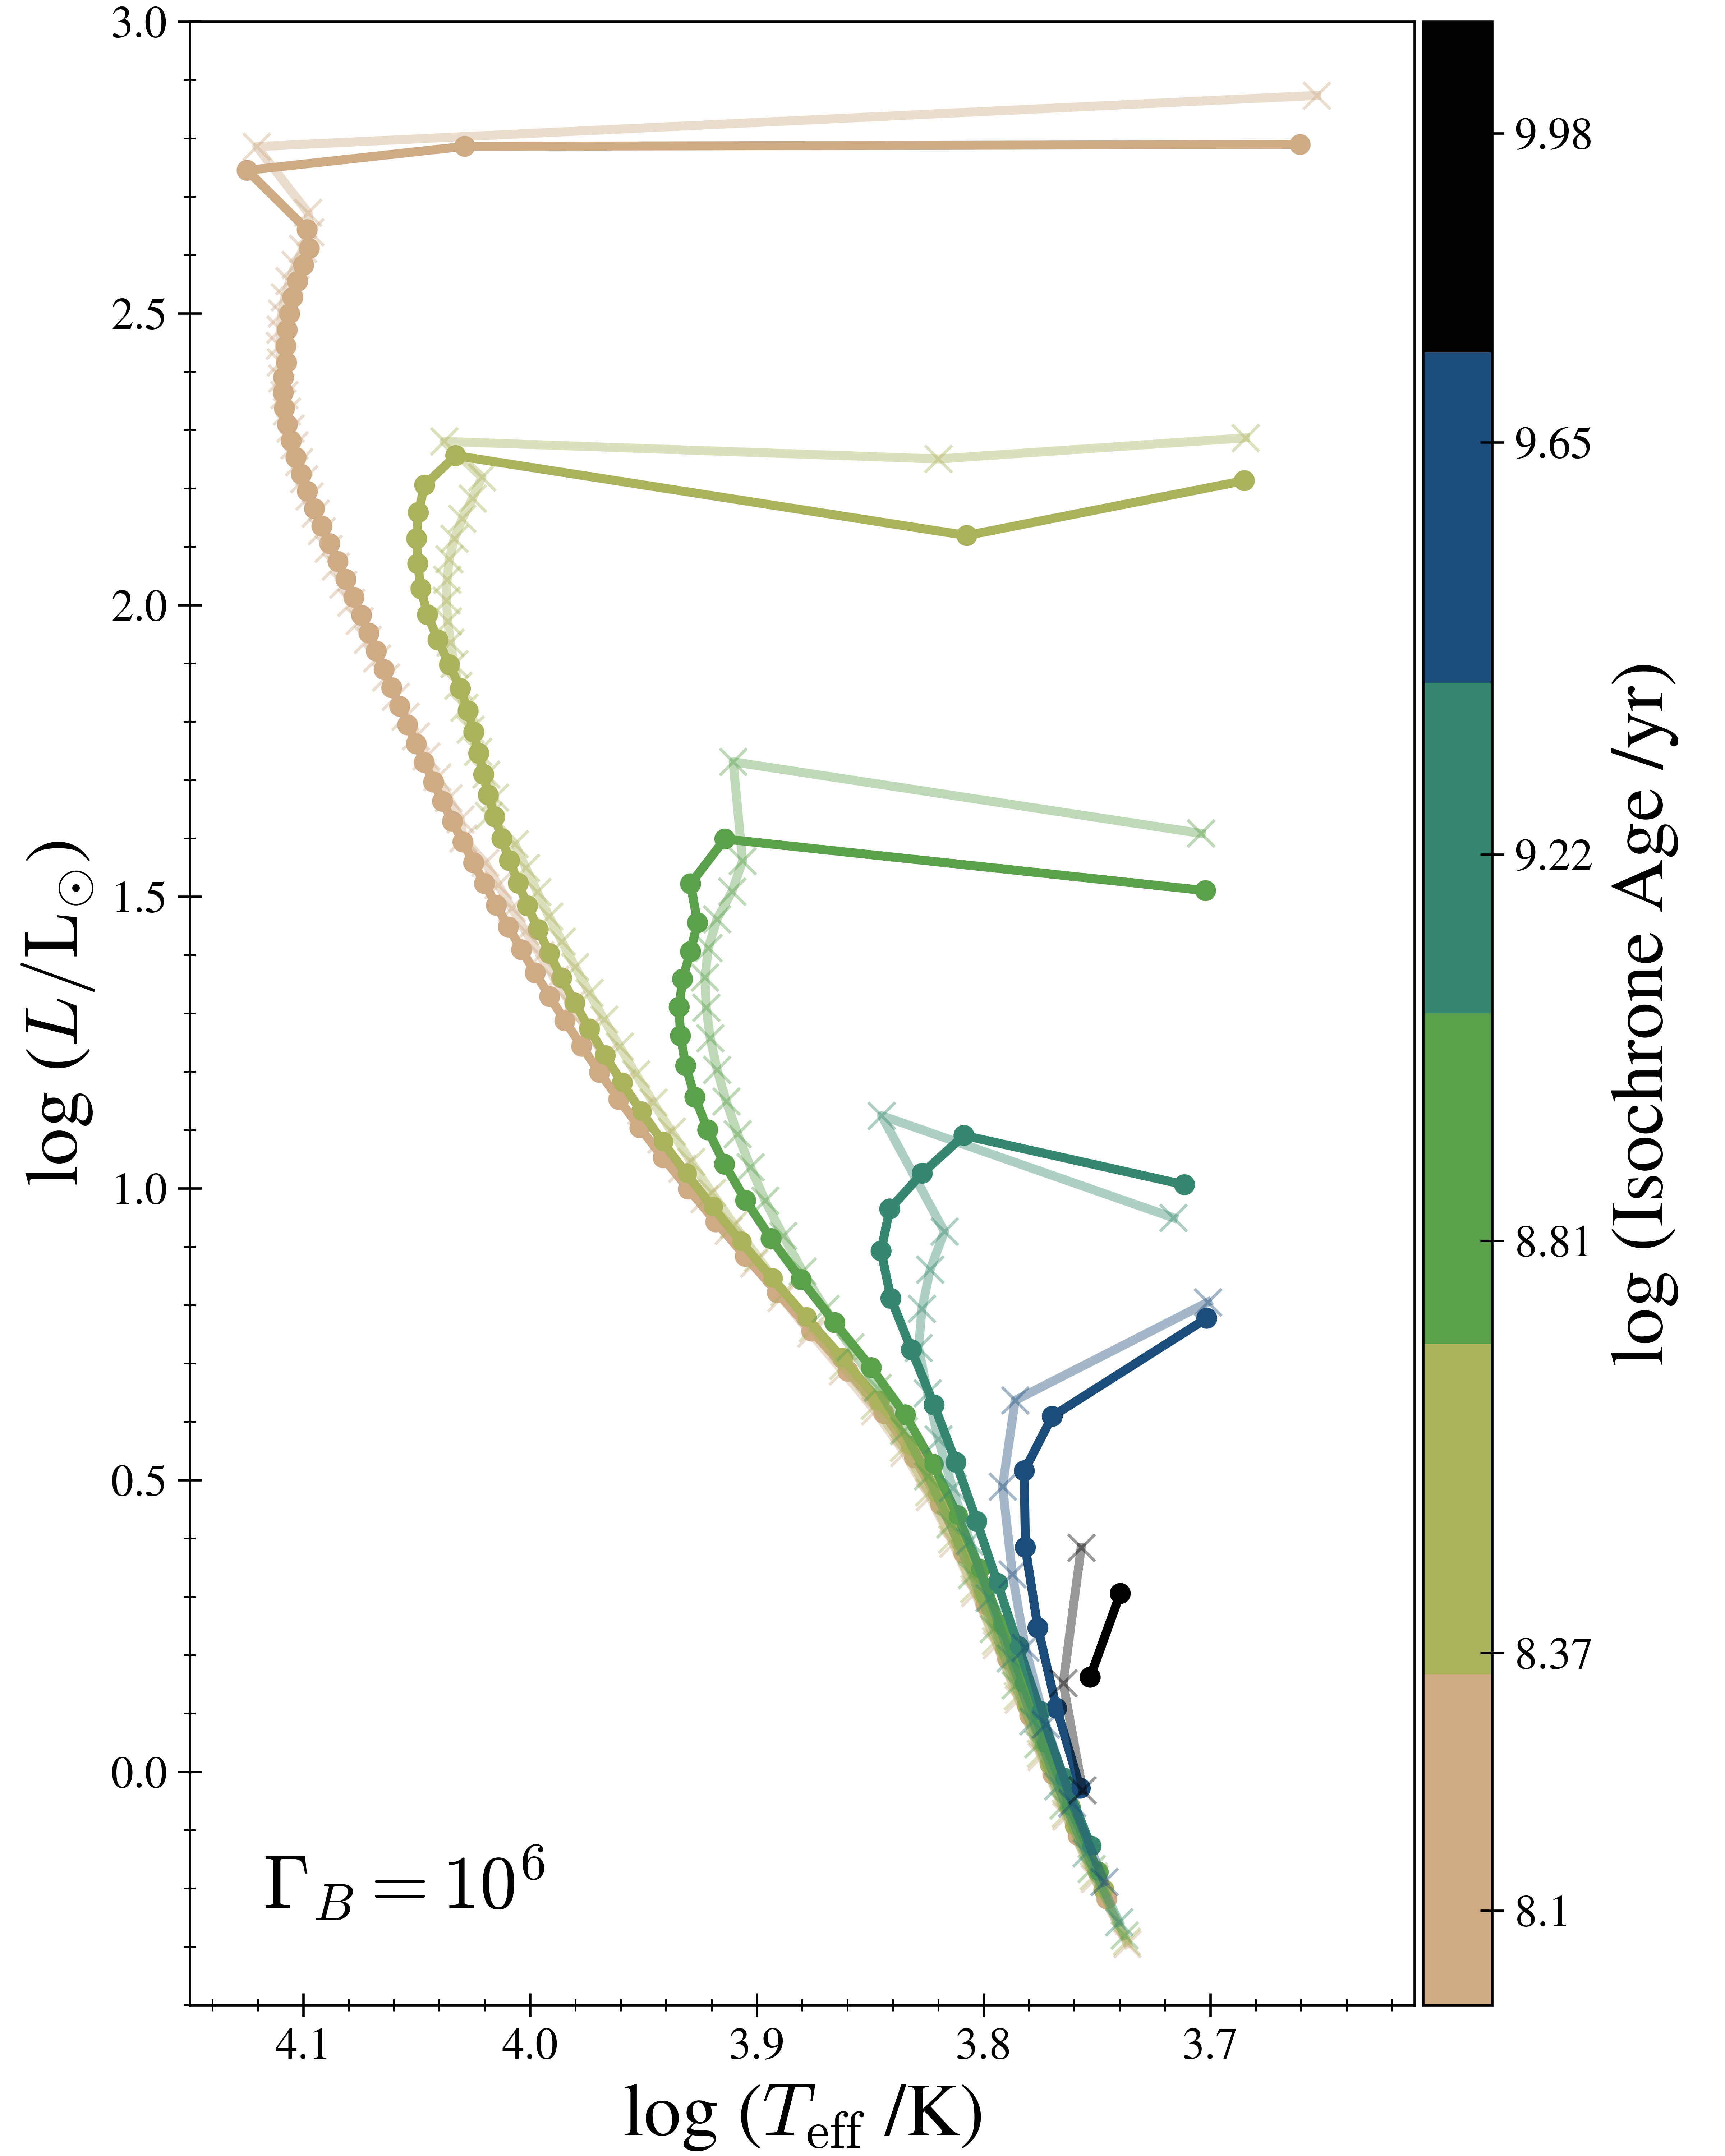
\includegraphics[width=\textwidth]{plots/isos_cb6.png}
  \caption{Same as Fig.~\ref{fig:isos_cb4} but for $\gbpow{6}$. The MS turnoff of isochrones between (insert ages) happens at a lower luminosity and skips the convective hook, causing them to appear older relative to \nodm isochrones.
  }
  \label{fig:isos_cb6}
\end{figure*}


% MS turnoff (hottest MS star) Teff and L plots
\begin{figure*}
    \centering
    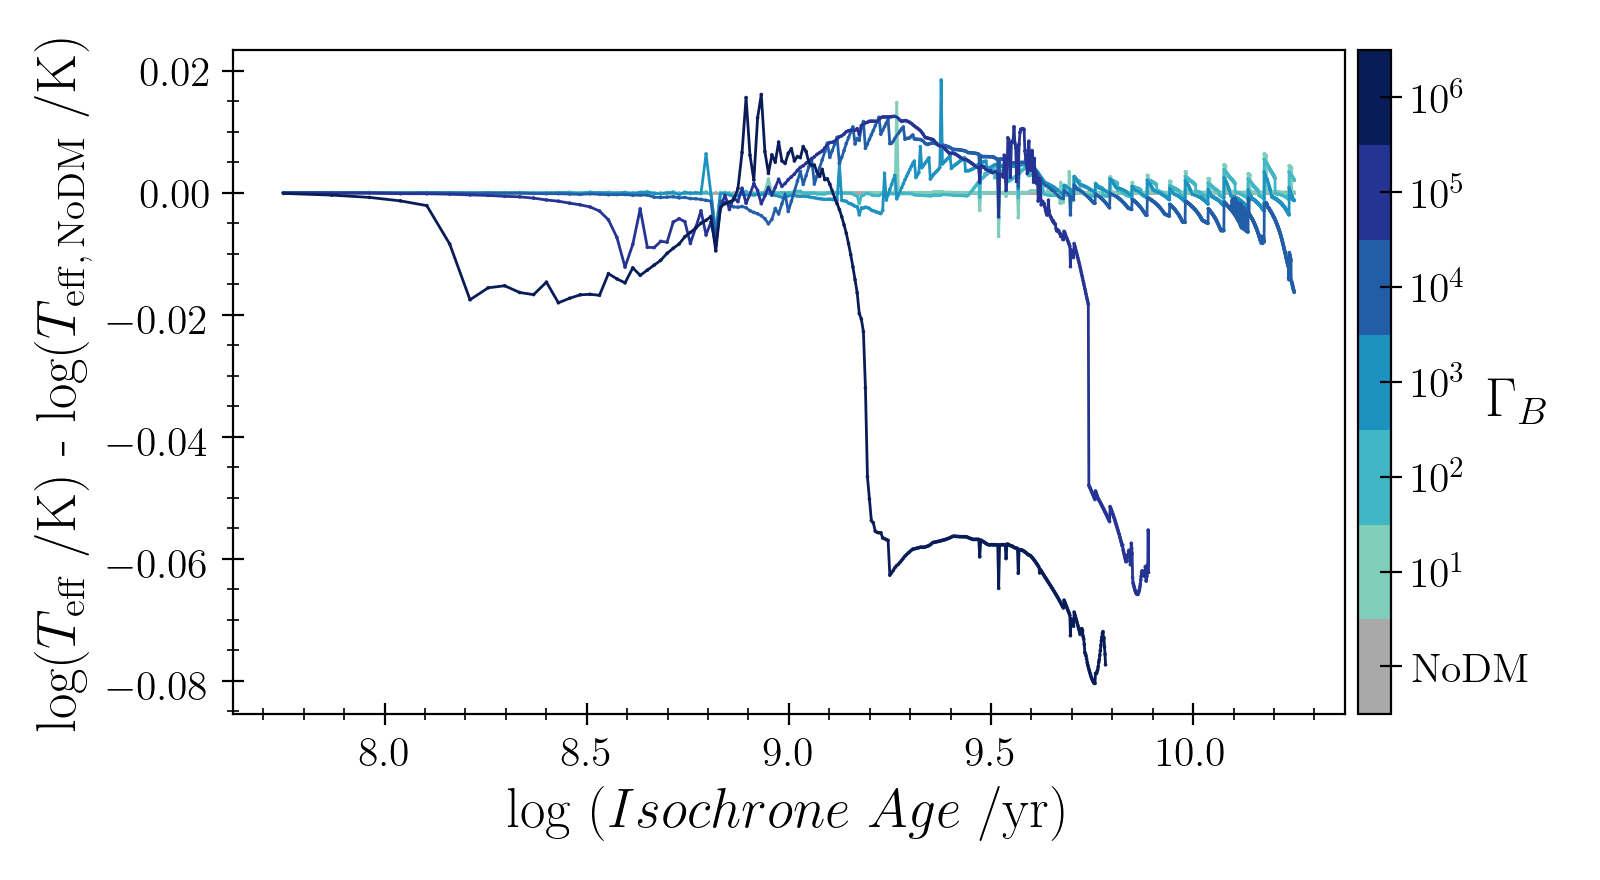
\includegraphics[width=\textwidth]{plots/hotTeff_resid.png}
    \caption{ PLACEHOLDER for MS turn off plots, Teff and/or L.
    Main sequence turnoff temperature (temperature of the hottest star that is still on the main sequence). Residuals are with respect to (...?)
    }
    \label{fig:hotTeff}

\end{figure*}


The isochrones in Figures~\ref{fig:isos_cb4,fig:isos_cb6} show the effects of ADM on the observable properties of stellar populations at fixed age (I know that L and Teff are not technically observable.. how do I re-word this?).

We find that, for stars significantly affected by ADM energy transport, the general effect is to shorten MS lifetimes so that, for a stellar populations of a given age, the MS turn-off happens at a lower mass and the stars evolve through the sub-giant branch at a lower luminosity. This causes isochrones of clusters in high $\gb$ environments to appear older than their standard model counterparts. This becomes noticeable in the highest $\gb$ environments around 0.2 Gyr as stars with $\rm{M} \approx 4 \Msun$ begin to leave the MS. Prior to this the stars have not had enough time to capture a sufficient number of DM particles for ADM-driven energy transport to be a significant contribution to the overall energy transfer within the stars.

Younger \nodm isochrones display a sharp feature called the convective hook near the MS turnoff, which is noticeably absent from the $\gbpow{6}$ isochrones. Since the \nodm models have convective cores, hydrogen is depleted nearly simultaneously throughout the volume of the core at the end of the MS. This causes the burning rate to decrease dramatically, which reduces the pressure support and results in gravitational contraction. The contraction increases the temperature until the bottom layer of hydrogen (now in a shell surrounding the core) is hot enough to ignite, reestablishing the pressure support. Our high $\gb$ isochrones lack this convective hook because ADM shuts off core convection. This lack of mixing causes the hydrogen to deplete first at the very center, and the burning gradually shifts into a shell, avoiding the sudden instability that causes the convective hook. This gradual shift to shell burning is very similar to the low mass \nodm models (which also do not experience a convective hook), which contributes to the high $\gb$ appearing older.

The gaps in the data are due to difficulty interpolating masses at a fixed time. Stellar masses generally increase when following a single isochrone from bottom to top. To build the isochrones from MESA's stellar models, MIST identifies the ages at which each star reaches a series of evolutionary milestones, and interpolates the stellar mass to generate properties of a group of stars at a fixed age. More massive stars generally evolve more quickly, and so the mapping between age and mass at a fixed milestone is usually monotonic, which the interpolation relies on. Exceptions to the monotonicity occur in mass regions where slightly less massive stars evolve more quickly. For example, in \nodm models, the emergence of a convective core around $1.3 \Msun$ results in stars just above this threshold living slightly \textit{longer} than stars just below it. With large amounts of ADM, the increase in stellar lifetimes through this transition to a convective core is much larger than in \nodm models and occurs over a wider mass range. These regions are not interpolated and appear as "missing" data in the isochrones.

Paragraph(s) on MS turnoff plots (Teff and/or L as fnc of isochrone age)


%------------------------------------------
\section{Discussion and Conclusions}
\label{sec:discus}

  Possible work for future: 1. vary DM mass and cross section (given observational constraints) to see how quick the effects vanish. 2. model iso curves and quantify how much older they look.


  %--------------------


  %--------------------
  % % m1p0 c0 kipp
  % \begin{figure*}
  % \centering
  %   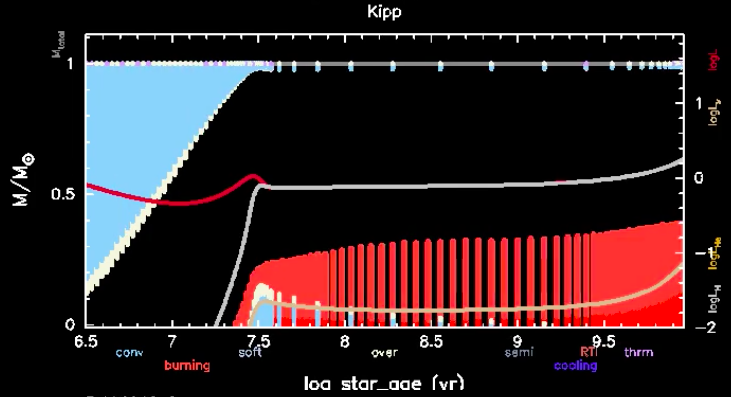
\includegraphics[width=\textwidth]{plots/m1p0c0_kipp.png}
  %   \caption{\label{fig:m1p0c0_kipp}Star mass 1.0Msun, c0, Main sequence burning. Note that the burning (shaded in red, left axis) doesn't extend as far as c6 model.}
  % \end{figure*}
  %--------------------

  %  \tjr{why are they destabilized? centerRho is higher, centerT is lower, Tmax-Tc is lower than lower cboosts (except extreme oscillations), oscillations start before Tc-Tx<0. what makes it go from transporting energy away from center to transporting to center? temp profile flattens (inverts? but cb<5 also invert so why are they still stable? they transport more energy than epsnuc. yes, oscillations turn on more slowly in c5, stable at $\epsilon_{\rm{x}}(r=0) \approx \epsilon_{\rm{nuc}}(r=0)$ for beginning of MS)}

  % The PP chain is less efficient? NO! PP, CNO have same net energy per pp fusion.

  % Nx and nxcenter are higher here than high mass stars, but wimps transport less heat here. why? Tx-Tc is much lower. but they still have a larger effect than in high mass stars because there is less energy flux to carry.

  % --------
  % 1.0 pgstar notes:
  % what i think is happening:
  % temp is lower so burning rate is much lower.
  % wimps take kinetic energy from protons. transport all of the energy generated from burning plus additional kinetic energy. burning rate goes down. temperature goes down.
  % temp and burning rate are still high (higher than c0?) in a shell where wimps have been depositing the energy. temp inverts and wimps start moving energy back to core (largest deltaT just before this happens?). proton kinetic energy goes up (so they are more likely to fuse when colliding) and burning rate goes up (largest deltaT here? no.).
  % 2 energy sources increase so temp goes up. temp no longer sufficiently inverted, wimps start moving energy away from core and process starts over.

  % stabalizes with large T inversion (deltaT=7.13-7.19 =4e-2) when degeneracy becomes important.

  % at center unless otherwise specified:
  % General oscillation pattern:
  % xheat negative and decreasing
  % burning, temp, and R decreasing, deltaT O(5e-4)
  % xheat peaks low, stays close for awhile

  % at 58 secs:
  % xheat, burning, temp all decreasing
  % TMR increasing, R decreasing

  % xheat peaks low at -80 (deltaT=7.0660-7.0656= 4e-4) then goes up
  % burning peaks low at 11 (TMR peaks high at same time or slightly before) then goes up
  % T peaks low at 7.0567 (deltaT=7.0573-7.0567 =6e-4) then goes up

  % xheat increases past 0 (deltaT=7.0582-7.0576= 6e-4)
  % luminosity goes negative at 0.08Msun
  % deltaT increasing

  % xheat peaks at 130 (deltaT=7.0711-7.0695= 16e-4) then oscillates up and down a bit
  % after last xheat peak, burning peaks at 20 then goes down
  % deltaT decreasing

  % xheat decreases past 0 (deltaT=7.0777-7.0771 =6e-4)
  % T peaks at 7.0772 (deltaT=7.0777-7.0772 =5e-4) then goes down
  % luminosity to zero (non-negative)

  % xheat peaks low at -100 (deltaT=7.0725-7.0722 =3e-4) then oscillates up and down a bit
  % after last xheat peak, burning peaks low at 11 then goes up
  % T peaks low at 7.0553 (deltaT=7.0558-7.0553 =5e-4)

  % xheat increases past 0 (deltaT=7.0569-7.0562 =7e-4)
  % luminosity goes negative at 0.08Msun

  % earlier:
  % xheat, burning, temp all decreasing
  % xheat peaks low at -40 then goes up
  % burning peaks low at 12 then goes up
  % T peaks low at 7.0592 then goes up

  % burning peaks at 14.5
  % xheat crosses 0, decreasing
  % T peaks high at 7.0664
  % burning decreasing
  % temp decreasing

  % temp is inverted
  % burning increasing
  % xheat positive
  % core radius is shrinking
  % R increasing

  % center temp increases, still inverted
  % xheat positive and decreasing
  % burning peaks
  % xheat goes negative
  % burning decreases

  % 1.0 pgstar notes end
  % --------


  % Stars leave the main sequence at a lower luminosity, which continues through the sub-giant branch (since He core mass is lower?), and the convective hook disappears. Caused by: lower gradT => lower central burning (CNO temp dependence) => core convection turns off => transition to H shell burning is more gradual.


\section{Discussion and Conclusions}
\label{sec:conclusions}

  \arz{I think that most of your conclusions section could be (1) a summary of our results and (2) speculations on how to turn this into a constraint in the future.}

\section*{Acknowledgements}



%%%%%%%%%%%%%%%%%%%%%%%%%%%%%%%%%%%%%%%%%%%%%%%%%%

%%%%%%%%%%%%%%%%%%%%%%%%%%%%%%%%%%%%%%%%%%%%%%%%%%

%%%%%%%%%%%%%%%%%%%%%%%%%%%%%%%%%%%%%%%%%%%%%%%%%%

%%%%%%%%%%%%%%%%%%%% REFERENCES %%%%%%%%%%%%%%%%%%

% The best way to enter references is to use BibTeX:

\bibliographystyle{mnras}
\bibliography{references}

%%%%%%%%%%%%%%%%%%%%%%%%%%%%%%%%%%%%%%%%%%%%%%%%%%

%%%%%%%%%%%%%%%%% APPENDICES %%%%%%%%%%%%%%%%%%%%%

% \appendix

% \section{section}
% \label{sec:sec}



%%%%%%%%%%%%%%%%%%%%%%%%%%%%%%%%%%%%%%%%%%%%%%%%%%



% Don't change these lines
\bsp	% typesetting comment

\label{lastpage}

\end{document}

% End of mnras_template.tex
